\section{Verificación de la suite de simulación}

En este capítulo se verán resultados en base a la elección de parámetros y datos de un CubeSat operativo, para obtener los MoP de apuntamiento con sus respectivos costos según los niveles de componentes físicos impuestos dentro de la simulación. Para ello, se define la cuantificación de los MoP de apuntamiento, se entregan los parámetros orbitales y se observan los valores obtenidos.

\subsection{Cuantificación de los MoP de apuntamiento}

Para lograr una capacidad de apuntamiento óptima, se debe considerar los MoP de apuntamiento. El apuntamiento se define como la capacidad que tiene el CubeSat para orientar la carga útil hacia un objetivo en específico, el cual, para este proyecto, será la tierra al imponer misiones del tipo observación terrestre. Teniendo esto en cuenta, existen índices de rendimiento con los cuales se verifica si este apuntamiento del satélite fue un éxito o un fracaso. Estos fueron revisados y descritos cualitativamente en \cite{ref6}, y debido a una revisión bibliográfica más extensa en libros sobre diseño de ADCS, se corrigieron y se cuantificaron, quedando como se muestra a continuación:

\underline{Exactitud de apuntamiento \cite{ref5,ref7}}

Es el índice con mayor relevancia dentro de las misiones de observación terrestre y de apuntamiento en general. Se refiere al error absoluto de apuntamiento del satélite, por lo que es la capacidad del CubeSat de mantener y controlar su orientación hacia una sección especifica de la Tierra. Esta se mide en termino de grados sexagesimales [°] o radianes [rad] y se notará dicho valor como la resta entre la orientación deseada del CubeSat y la posición obtenida mediante el ADCS, sabiendo que existen posibles errores de determinación de actitud o de actuadores que no puedan ejercer el torque requerido.

\underline{Jitter \cite{ref5,ref9,ref10}}

El Jitter en la línea de visión (LoS, por sus siglas en inglés) de la nave espacial se define como las vibraciones mecánicas sinusoidales de pequeña amplitud que ocurren debido a las interacciones dinámicas causadas por dispositivos mecánicos vibratorios montados en la nave espacial o dentro del instrumento (s) de carga útil y que aparecen a frecuencias en o por encima del ancho de banda del Attitude Control System (ACS) del satélite, desde unos pocos Hz hasta cientos de Hz, y que perturban indeseablemente el apuntamiento de la línea de visión de la carga útil. Para visualizar este problema, se debe revisar si existen en las sinusoidales alrededor del eje de equilibrio a controlar en los ángulos de Euler, leves perturbaciones asemejadas al ruido, que representan la inestabilidad del satélite al tomar diferentes orientaciones pequeñas en bajos periodos de tiempo, que hacen que la cámara sea vea “empañada”. Para representar dicho problema, se considera la densidad espectral de potencia como una medida de cuantificación del jitter, el cual se obtendrá una vez fijado un filtro pasa alto de hasta una frecuencia adecuada (generalmente 10 [Hz]) aplicada a la respuesta obtenida. Se observará un alto nivel de jitter si existe un valor de la densidad espectral de potencia mayor, al consumir más energía en dicho rango de frecuencias.

\underline{Agilidad \cite{ref5, ref11}}

Se refiere a lograr una maniobra de actitud mínima, el cual es una combinación de apuntar al objetivo (sección de la Tierra) en el menor tiempo posible a través de una maniobra de giro. En otras palabras, se busca que el CubeSat intercepte al objetivo lo más rápido posible y mantenga la orientación en una exactitud de apuntamiento aceptable dentro de los requerimientos. Para cuantificar este índice, se hará uso del parámetro del tiempo de asentamiento (Settling Time), el cual especifica el tiempo permitido para recuperarse de maniobras o perturbaciones. Si existe un tiempo de asentamiento menor en alguna comparación de dos ADCS, sería más ágil aquel que presente un menor tiempo de asentamiento, comparándolo a través de una gráfica de velocidad angular respecto al tiempo, asumiendo una banda de asentamiento adecuada.

\underline{Drift \cite{ref5}}

Se refiere a cuánto puede desviarse un vehículo con el tiempo. Este parámetro es crucial cuando se necesita mantener una dirección específica y se deben hacer correcciones solo ocasionalmente para evitar que el vehículo se desvíe significativamente de su curso deseado. Representado mediante ángulos por hora [°/hr]

Para el caso de este análisis de la suite de simulación, se consideraron solo las tres primeras. El Drift solo se menciona, pero no se cuantifica en este trabajo.

\subsection{Condiciones y parámetros de simulación}

Para obtener resultados de rendimiento, se utilizaron los datos de TLE del SUCHAI-3 con fecha de inicio del 01 de noviembre del 2023, que son las mismas condiciones iniciales utilizadas en el Capítulo 4 para visualizar el SGP4 y los modelos orbitales en ECI (IGRF y vector sol). Se debe tener en cuenta que estas condiciones, en conjunto con otros parámetros son dados para todos los niveles de sensores y actuadores impuestos dentro de la suite de simulación, y sirven para tener un parámetro comparativo entre los componentes físicos del ADCS.

En la Tabla~\ref{tab:parametros} se muestran los valores de los parámetros recién mencionados utilizados en la simulación, que son basados en literatura \cite{ref14,ref41,ref44} o por elaboración propia. Cabe mencionar que $q_i$ y $\omega_i$ representan la orientación y velocidad angular inicial real.

\begin{table}[h!]
	\centering
	\caption{Parámetros del sistema}
	\begin{tabular}{|c|c|}
		\hline
		\textbf{Parámetro} & \textbf{Valor} \\
		\hline
		$[I_x, I_y, I_z] \ [kg \cdot m^2]$ & $[0.037, 0.036, 0.036]$ \\
		\hline		
		$[I_{s0}, I_{s1}, I_{s2}] \ [kg \cdot m^2]$ & $[0.005, 0.005, 0.004]$ \\
		\hline
		$[b_0, b_1, b_2] \ [m]$ & $[0.05, 0.05, 0.015]$ \\
		\hline		
		$\omega_{0,0} \ [rad/s]$ & $0.00163$ \\
		\hline
		$T_{\text{prop}} \ [s]$ & $345718 \ \text{[s]} \ (60 \ \text{órbitas})$ \\
		\hline
		$q_i \ [-]$ & $\left[ 0.0789, 0.0941, 0.0789, 0.9893 \right]$ \\
		\hline
		$\omega_i \ [rad/s]$ & $[0.0001, 0.0001, 0.0001]$ \\
		\hline
		$[\omega_{s0}, \omega_{s1}, \omega_{s2}] \ [rad/s]$ & $[0.00001, 0.00001, 0.00001]$ \\
		\hline
		$P_{i, \text{MT}}$ & $\text{diag}(0.25, 0.25, 0.25, 0.01, 0.01, 0.01)$ \\
		\hline
		$P_{i, \text{RW}}$ & $\text{diag}(P_{i, \text{MT}}, 0.001, 0.001, 0.001)$ \\
		\hline
	\end{tabular}

	\label{tab:parametros}
\end{table}

Además, con el objetivo de visualizar en el simulador el rendimiento de apuntamiento y su costo asociado, se decide agrupar los componentes físico en niveles según el COTS disponible en CubeSat~\cite{ref45}. Esto se hace debido a que existen una variedad considerable de componentes capaces de ser usado en este tipo de nanosatélites, al ser de poco costo tanto energético como monetario. Caracterizar todos estos se escapa de los objetivos del trabajo, ya que su consideración genera un análisis extenso e innecesario respecto a la obtención de los costos en base a los SE envelopes. Por ello, se presenta en la Tabla~\ref{tab:niveles} los componentes COTS seleccionados en conjunto con su proveedor para analizar tanto el rendimiento (MoP de apuntamiento) como el costo utilizado por cada uno de ellos. Mas detalles de cada uno de los sensores y actuadores elegidos en el Anexo C????.

\begin{table}[h!]
	\centering
	\caption{Componentes clasificados por nivel de rendimiento}
	\begin{tabular}{|c|c|c|c|}
		\hline
		\textbf{Componente}   & \textbf{Nivel bajo} & \textbf{Nivel medio} & \textbf{Nivel alto} \\ 
		\hline
		\textbf{Giroscopio}   & CRH03 - 200  & CRH03 - 010  & NSGY-001   \\
		& (Silicon Sensing  & (Silicon Sensing & (NewSpace \\
		& Systems) & Systems) & Systems) \\
		\hline
		\textbf{Magnetómetro} & Fluxgate Magnetometer & MM200-1 & MM200-2  \\
		& FGM-A-75 & (AAC Clyde Space) & (AAC Clyde Space) \\
		& (ZARM Technik) & & \\
		\hline
		\textbf{Sun Sensor}   & CSS-01, CSS-02  & MSS-01 & FSS  \\
		& (Space Micro)   & (Space Micro) & (Bradford Space) \\
		\hline
		\textbf{Magnetorquer} & MT0.5-1 & NCTR-M012 & MT15-1 \\
		& (ZARM Technik) & (NewSpace Systems) & (ZARM Technik) \\
		\hline
		\textbf{Rueda de reacción} & RWP500 & RW1  & RW4  \\
		& (Blue Canyon & (Blue Canyon & (Blue Canyon \\
		& Technologies) & Technologies) & Technologies) \\
		\hline
	\end{tabular}
	\label{tab:niveles}
\end{table}


Es relevante mencionar que en el Anexo H??? se muestra un ejemplo a detalle sobre la obtención de los MoP de apuntamiento, siendo estos los pasos a seguir para los casos de estudio que se mencionarán en las siguientes secciones.

\subsection{Resultados suite de simulación}

En esta sección se presentarán análisis respecto a los resultados obtenidos utilizando los parámetros de la sección anterior. Se compararan los diferentes niveles de sensores y actuadores, los tipos de actuadores y los controladores utilizados para conocer la performance y costo de cada caso.

\subsubsection{Resultados tipos de actuadores}



\begin{figure}[H]
	\centering    
	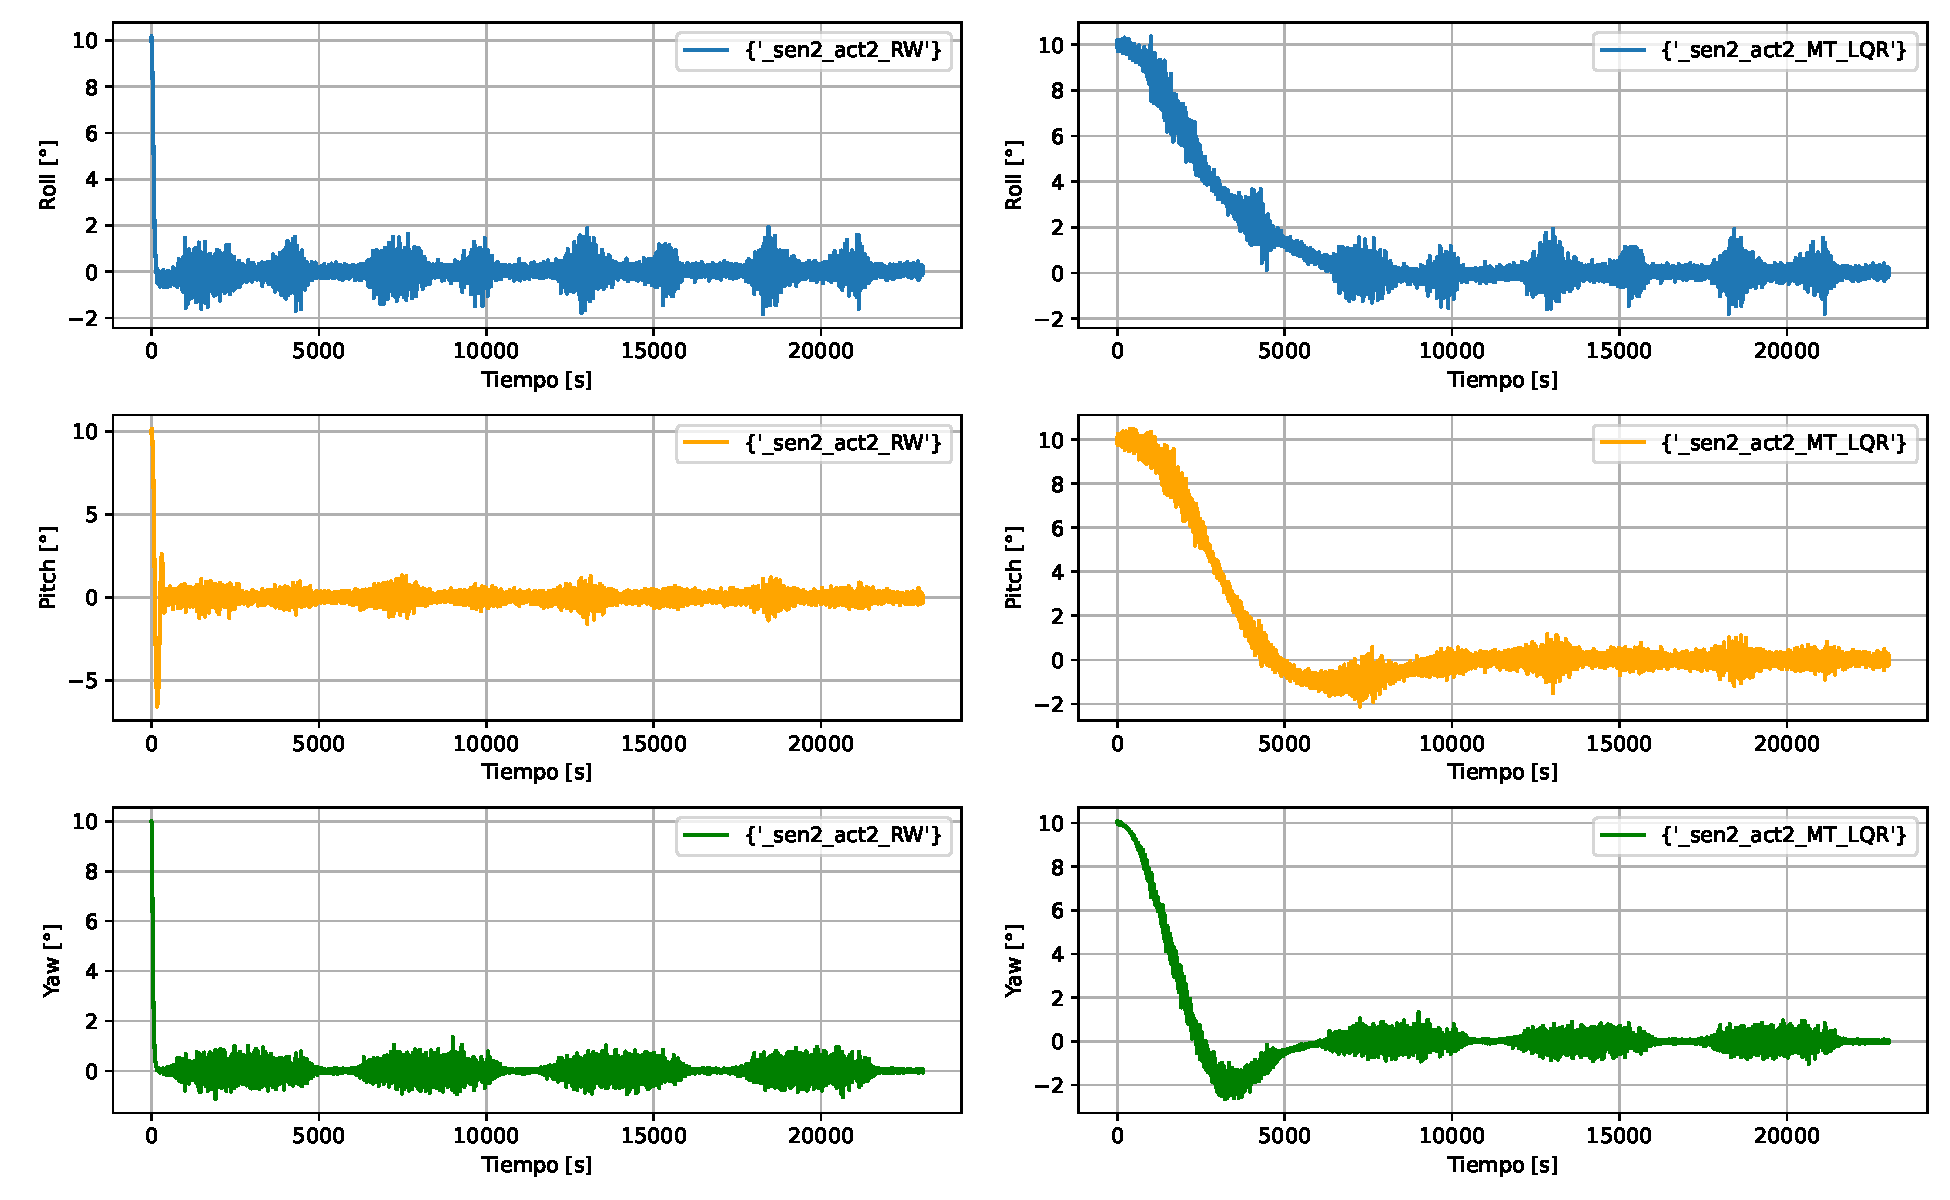
\includegraphics[width=0.97\textwidth]{MT_RW_nivel2.pdf}
	\caption{Ángulos de Euler LVLH y body para dos actuadores distintos (Elaboración propia).}
	\label{fig:MT_RW_nivel2}
\end{figure}


\begin{table}[h!]
	\centering
	\caption{Rendimiento y costo para rueda de reaccion y magnetorquer en mismas condiciones}
	\begin{tabular}{|c|c|c|c|c|c|}
		\hline
		\textbf{Tipo de}   & \textbf{Potencia} & \textbf{Masa [kg]} & \textbf{Accuracy [°]} & \textbf{Jitter} & \textbf{Agilidad [s]}  \\ 
		\textbf{actuador}   & \textbf{máxima [W]} & & & \textbf{[W/Hz]} &  \\
		\hline
		\textbf{Rueda de}   & 9  & 0.95  & 0.94 & 0.16 & 228   \\
		\textbf{reacción}   &  &   &  &  &    \\
		\hline
		\textbf{Magnetorquer}   & 0.8  & 0.053  & 1.71 & 0.42 & 3933   \\
		& & & & &   \\
		\hline
	\end{tabular}
	\label{tab:RW_MT_nivel2}
\end{table}


\subsubsection{Resultados de los controladores}

\begin{figure}[H]
	\centering    
	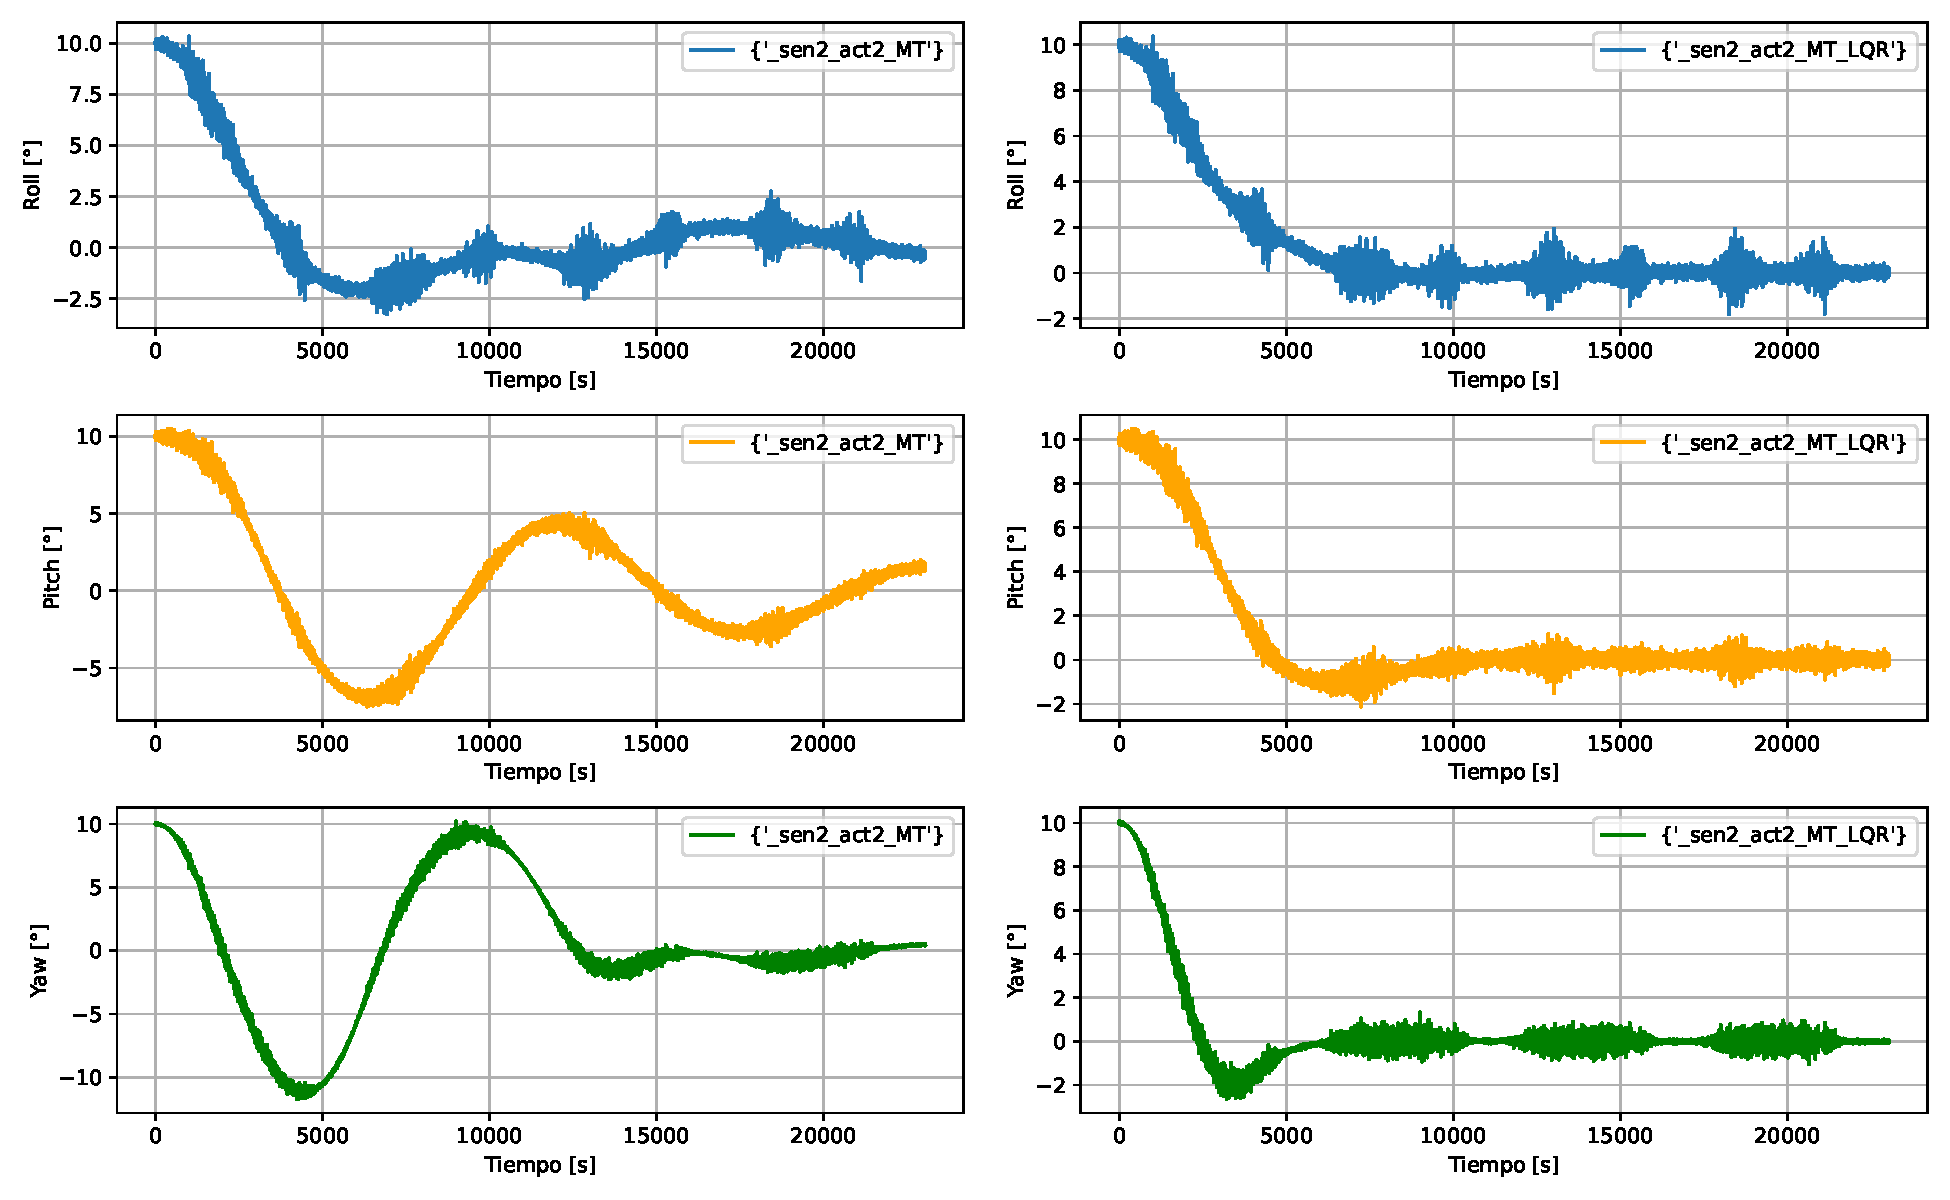
\includegraphics[width=0.97\textwidth]{PD_LQR_nivel2.pdf}
	\caption{Ángulos de Euler LVLH y body para dos controladores distintos (Elaboración propia).}
	\label{fig:PD_LQR_nivel2}
\end{figure}


\begin{table}[h!]
	\centering
	\caption{Rendimiento y costo para controlador PD y LQR en mismas condiciones}
	\begin{tabular}{|c|c|c|c|c|c|}
		\hline
		\textbf{Controlador}   & \textbf{Potencia} & \textbf{Masa [kg]} & \textbf{Accuracy [°]} & \textbf{Jitter} & \textbf{Agilidad [s]}  \\ 
		  & \textbf{máxima [W]} & & & \textbf{[W/Hz]} &  \\
		\hline
		\textbf{PD}   & 0.8  & 0.053  & 2.46 & 0.43 & 14040   \\
		&  &   &  &  &    \\
		\hline
		\textbf{LQR}   & 0.8  & 0.053  & 1.71 & 0.43 & 3933   \\
		& & & & &   \\
		\hline
	\end{tabular}
	\label{tab:PD_LQR_nivel2}
\end{table}

\subsubsection{Resultados niveles de sensores}

\begin{figure}[H]
	\centering    
	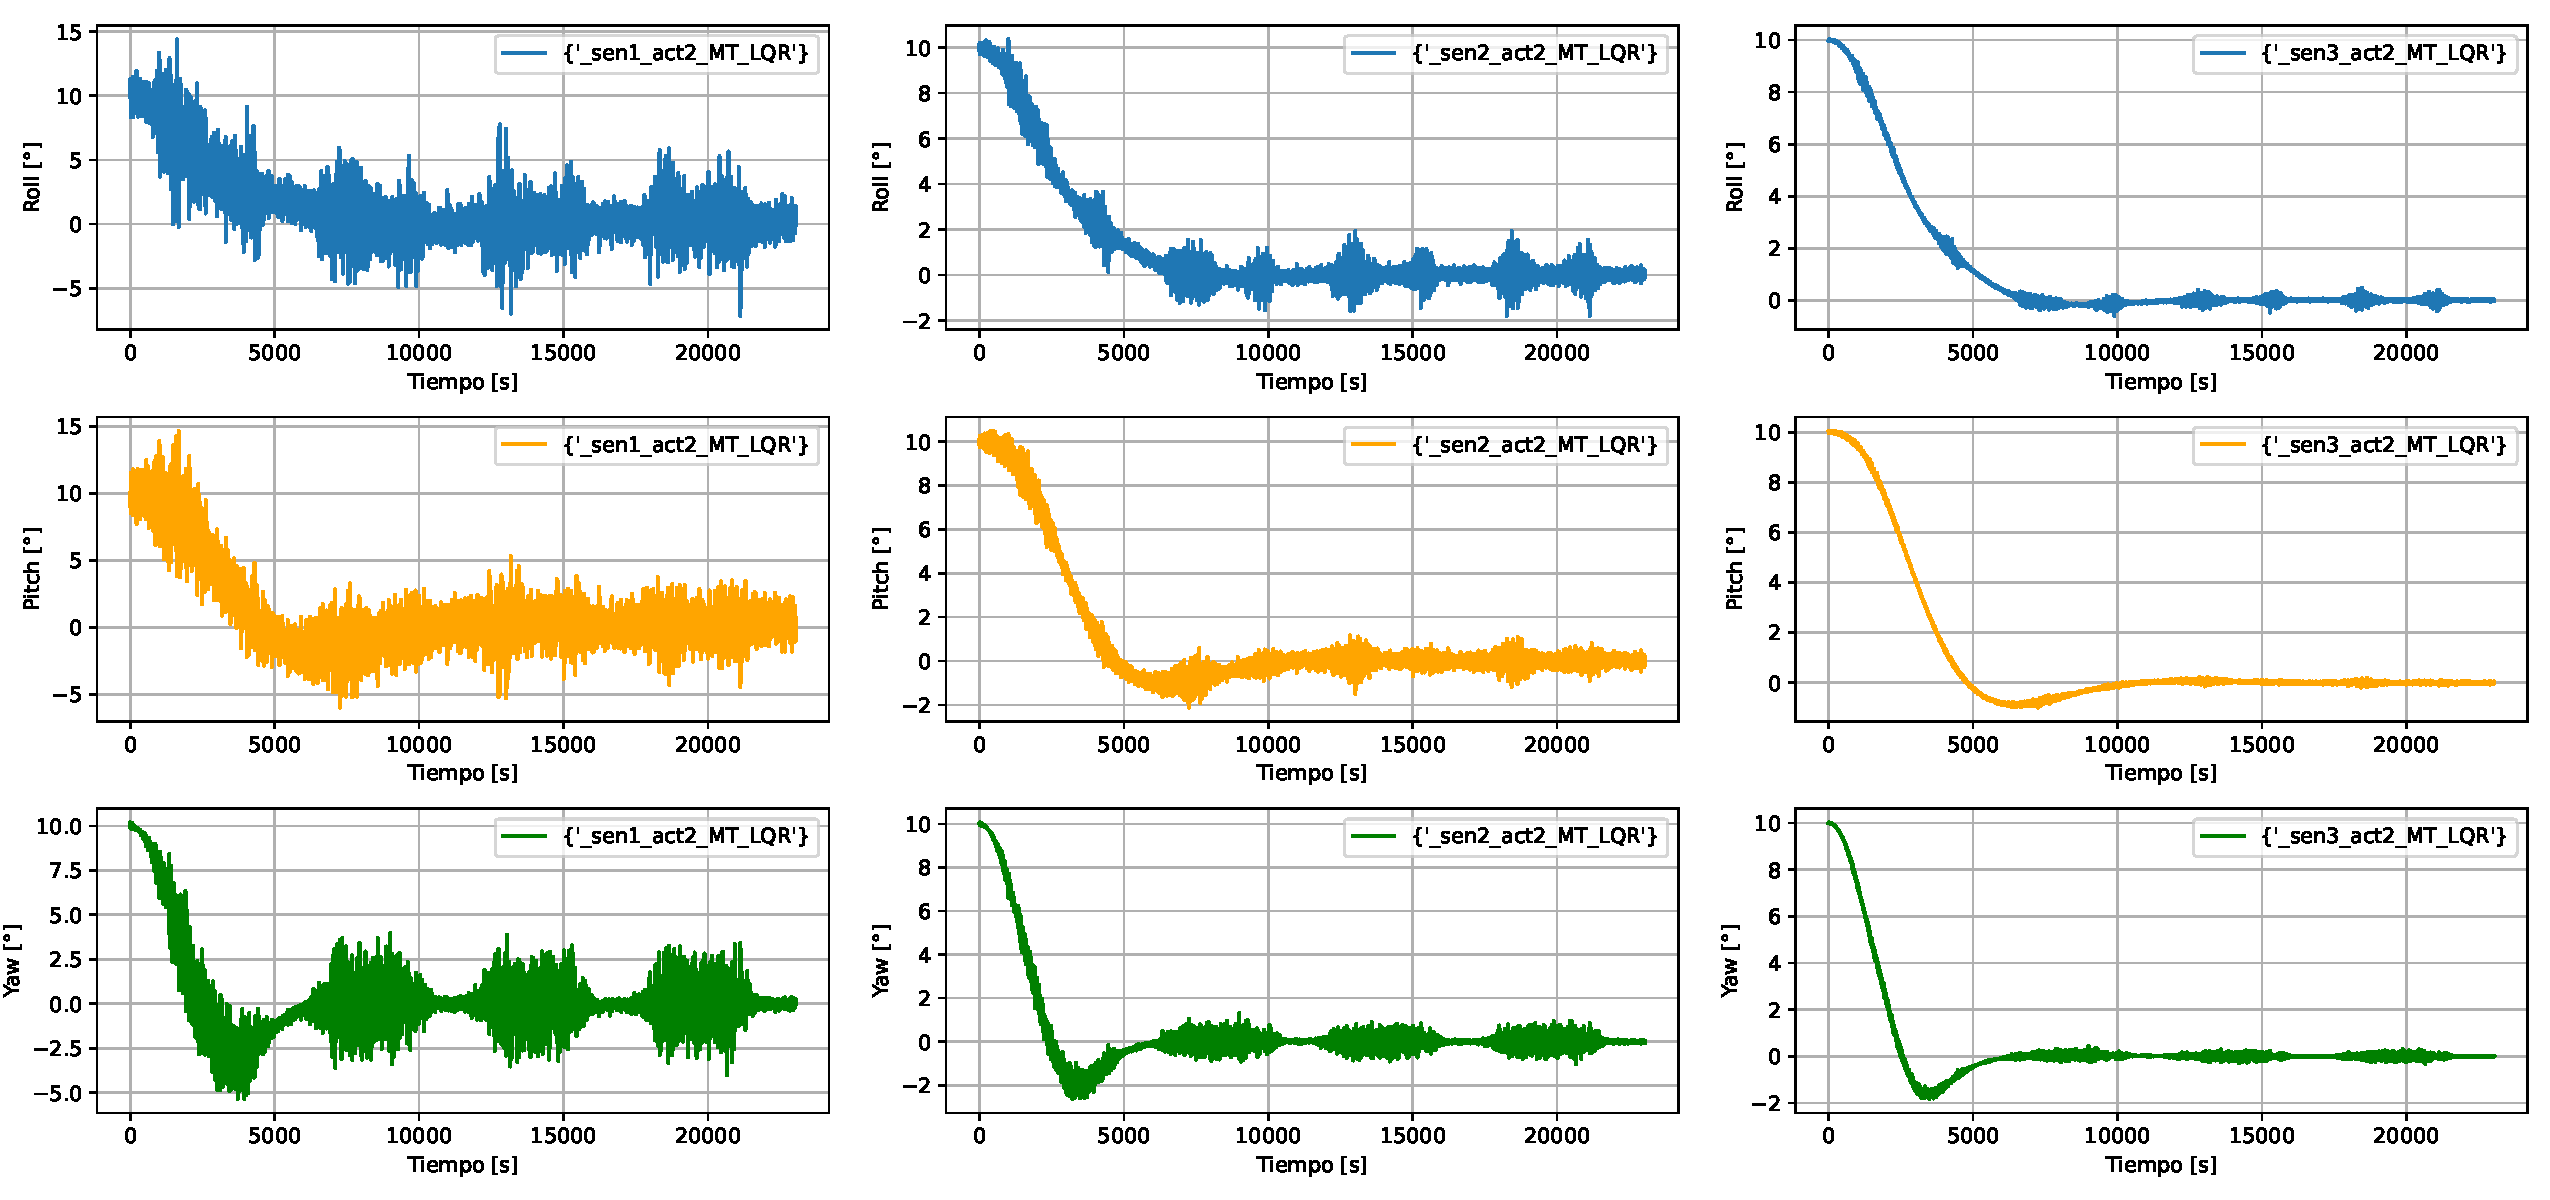
\includegraphics[width=0.97\textwidth]{MT_LQR_sensores.pdf}
	\caption{Ángulos de Euler LVLH y body para niveles de sensor distintos con magnetorquer (Elaboración propia).}
	\label{fig:MT_LQR_sensores}
\end{figure}


\begin{table}[h!]
	\centering
	\caption{Rendimiento y costo para niveles de sensor con nivel 2 de magnetorquer y LQR}
	\begin{tabular}{|c|c|c|c|c|c|}
		\hline
		\textbf{Nivel de}   & \textbf{Potencia} & \textbf{Masa [kg]} & \textbf{Accuracy [°]} & \textbf{Jitter} & \textbf{Agilidad [s]}  \\ 
		\textbf{sensor}  & \textbf{máxima [W]} & & & \textbf{[W/Hz]} &  \\
		\hline
		\textbf{Nivel 1}   & 0.15  & 0.067  & 3.72 & 2.92 & 4081   \\
		&  &   &  &  &    \\
		\hline
		\textbf{Nivel 2}   & 0.3  & 0.181  & 1.71 & 0.43 & 3933   \\
		& & & & &   \\
		\hline
		\textbf{Nivel 3}   & 0.75  & 0.530  & 1.5 & 0.43 & 3957   \\
		& & & & &   \\
		\hline		
	\end{tabular}
	\label{tab:MT_LQR_sensores}
\end{table}

\begin{figure}[H]
	\centering    
	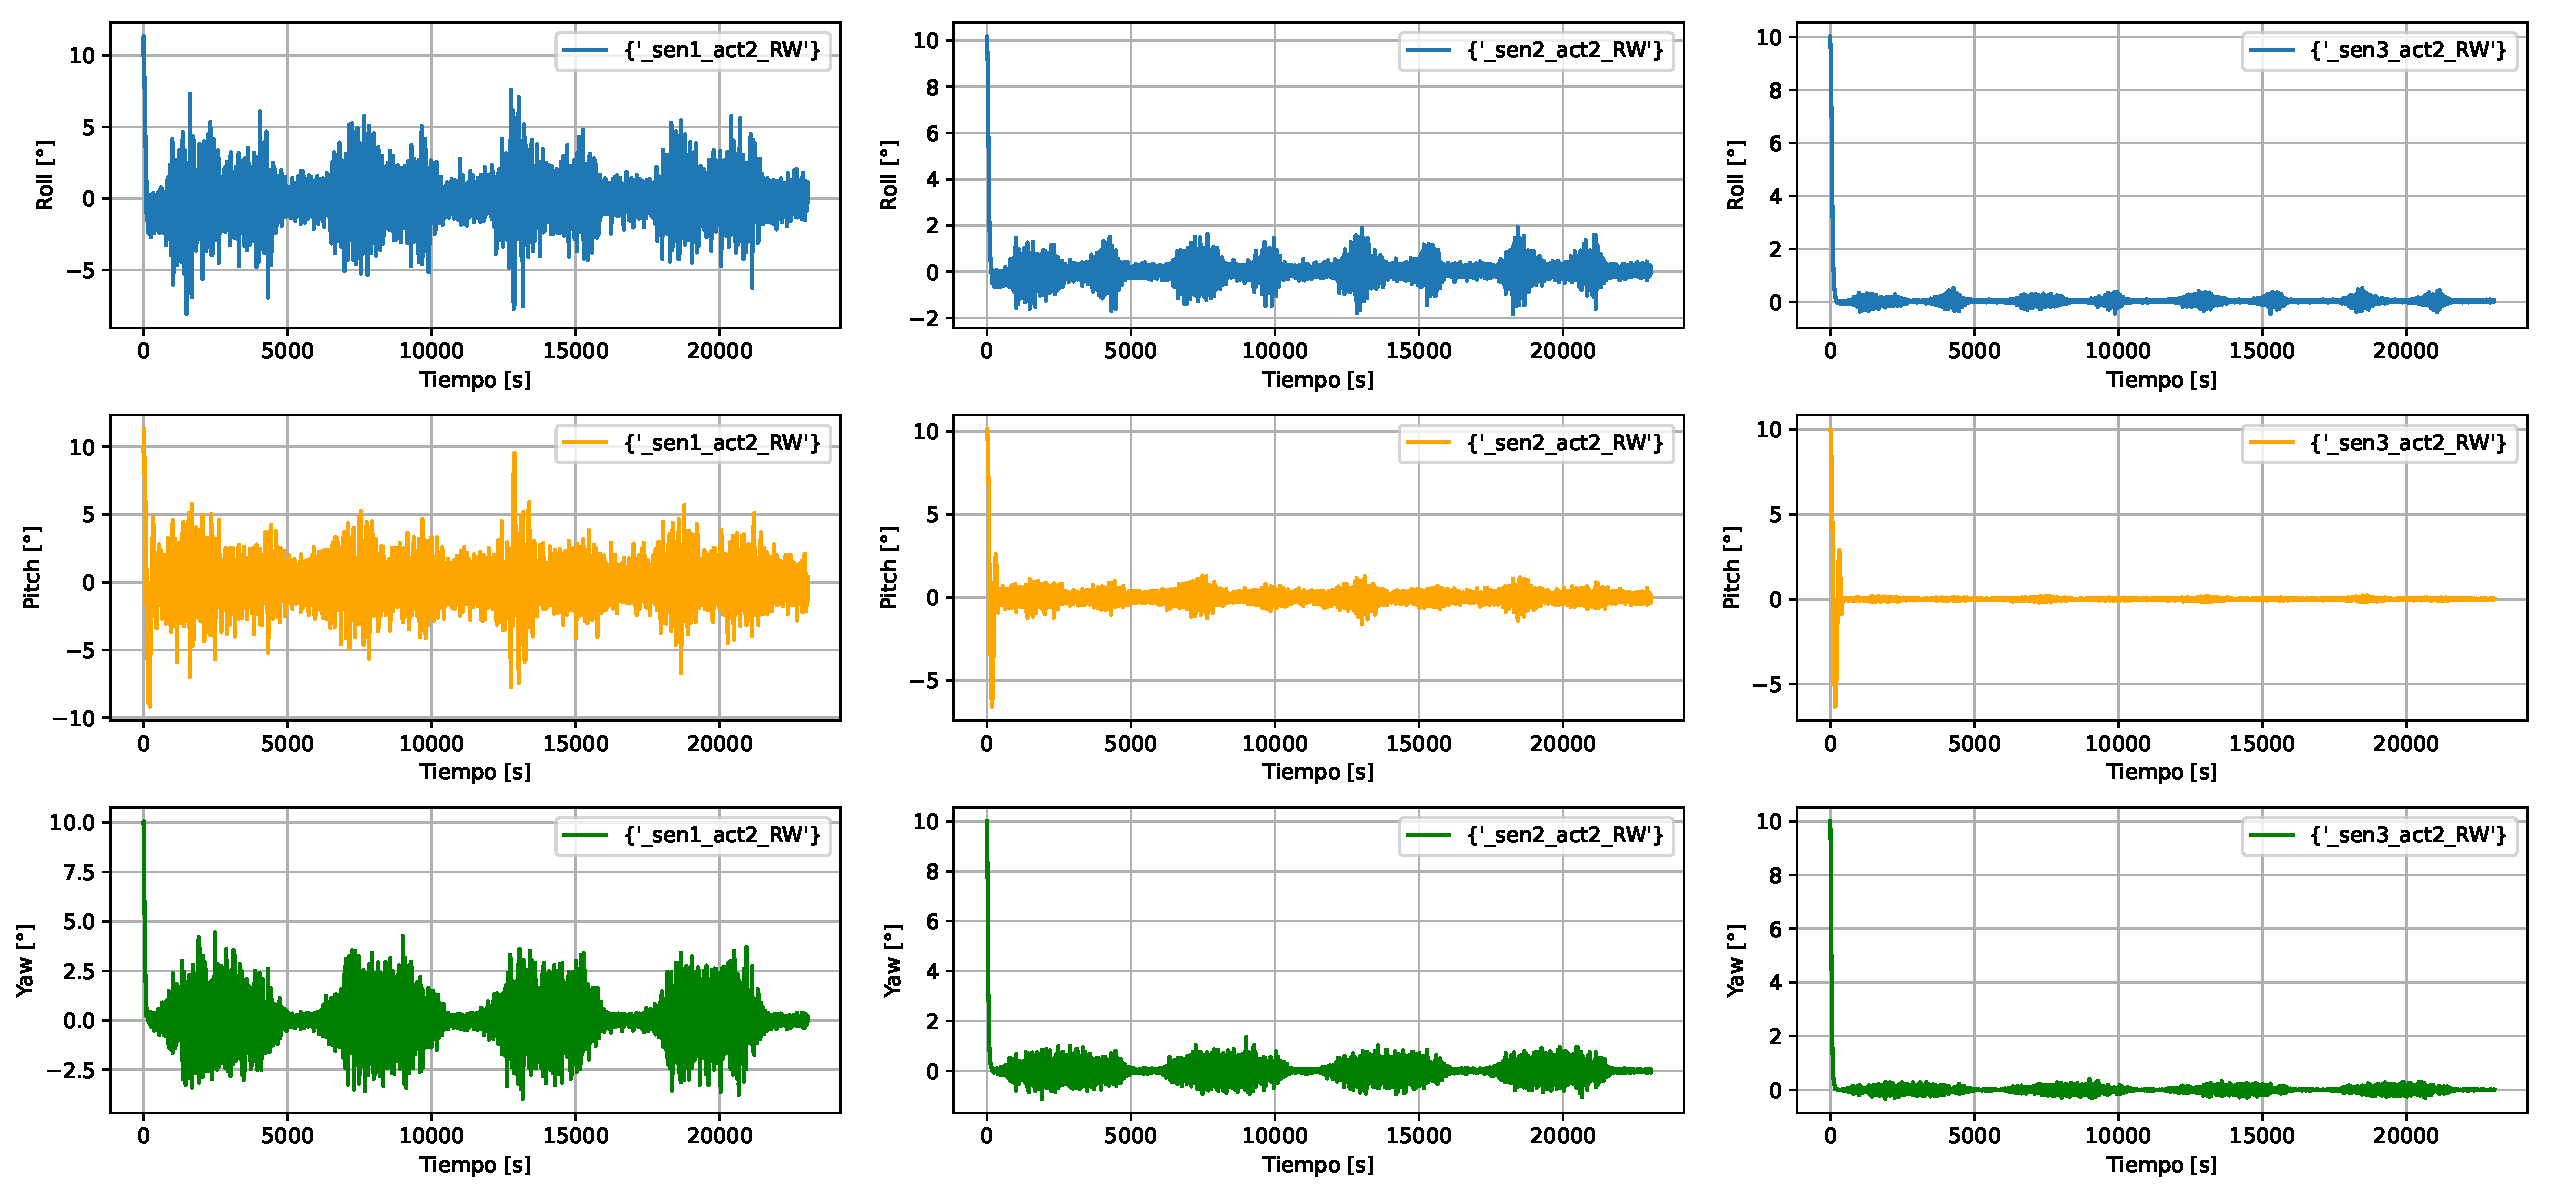
\includegraphics[width=0.97\textwidth]{RW_LQR_sensores.pdf}
	\caption{Ángulos de Euler LVLH y body para niveles de sensor distintos con rueda de reacción (Elaboración propia).}
	\label{fig:RW_LQR_sensores}
\end{figure}


\begin{table}[h!]
	\centering
	\caption{Rendimiento y costo para niveles de sensor con nivel 2 de rueda de reacción y LQR}
	\begin{tabular}{|c|c|c|c|c|c|}
		\hline
		\textbf{Nivel de}   & \textbf{Potencia} & \textbf{Masa [kg]} & \textbf{Accuracy [°]} & \textbf{Jitter} & \textbf{Agilidad [s]}  \\ 
		\textbf{sensor}  & \textbf{máxima [W]} & & & \textbf{[W/Hz]} &  \\
		\hline
		\textbf{Nivel 1}   & 0.15  & 0.067  & 3.76 & 3.28 & 230  \\
		&  &   &  &  &    \\
		\hline
		\textbf{Nivel 2}   & 0.3  & 0.181  & 0.93 & 0.16 & 228   \\
		& & & & &   \\
		\hline
		\textbf{Nivel 3}   & 0.75  & 0.530  & 0.52 & 0.02 & 229   \\
		& & & & &   \\
		\hline		
	\end{tabular}
	\label{tab:RW_LQR_sensores}
\end{table}

\subsubsection{Resultados niveles de actuadores}


\begin{figure}[H]
	\centering    
	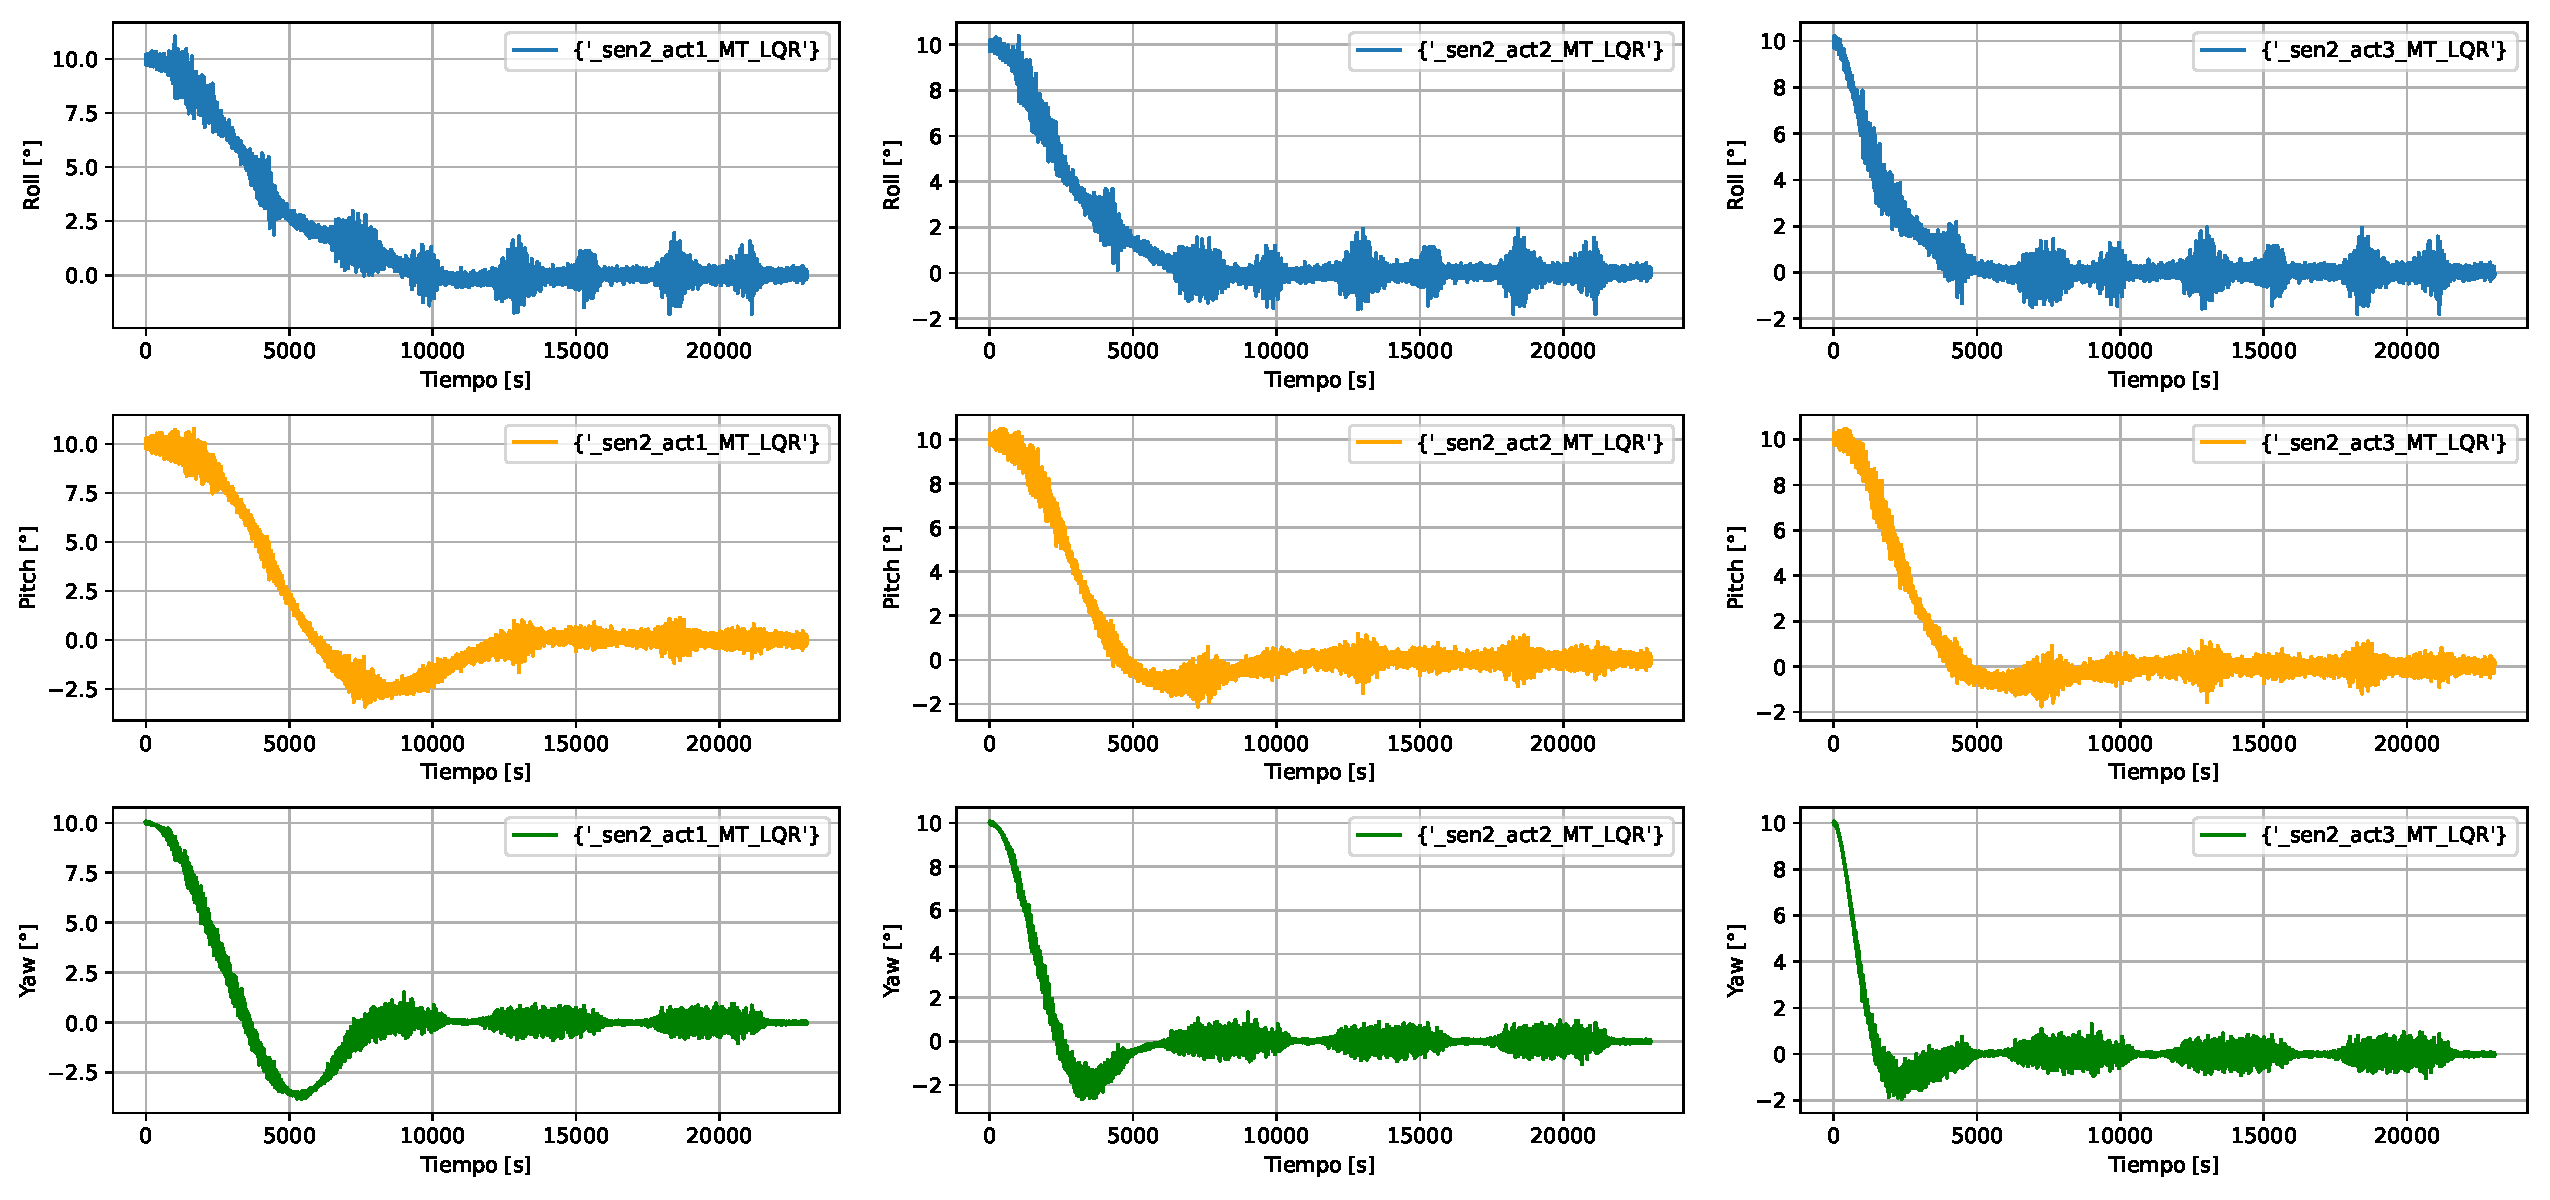
\includegraphics[width=0.97\textwidth]{MT_LQR_actuadores.pdf}
	\caption{Ángulos de Euler LVLH y body para niveles de magnetorquer distintos con sensores nivel 2 (Elaboración propia).}
	\label{fig:MT_LQR_actuadores}
\end{figure}


\begin{table}[h!]
	\centering
	\caption{Rendimiento y costo para niveles de magnetorquer con nivel 2 de sensor y LQR}
	\begin{tabular}{|c|c|c|c|c|c|}
		\hline
		\textbf{Nivel de}   & \textbf{Potencia} & \textbf{Masa [kg]} & \textbf{Accuracy [°]} & \textbf{Jitter} & \textbf{Agilidad [s]}  \\ 
		\textbf{actuador}  & \textbf{máxima [W]} & & & \textbf{[W/Hz]} &  \\
		\hline
		\textbf{Nivel 1}   & 0.275  &  0.03  & 3.09 &  0.41 & 5821   \\
		&  &   &  &  &    \\
		\hline
		\textbf{Nivel 2}   & 0.8  & 0.053  & 1.71 & 0.43 & 3933   \\
		& & & & &   \\
		\hline
		\textbf{Nivel 3}   & 1.11  & 0.43  & 1.83 & 0.49 & 2692   \\
		& & & & &   \\
		\hline		
	\end{tabular}
	\label{tab:MT_LQR_actuadores}
\end{table}

\begin{figure}[H]
	\centering    
	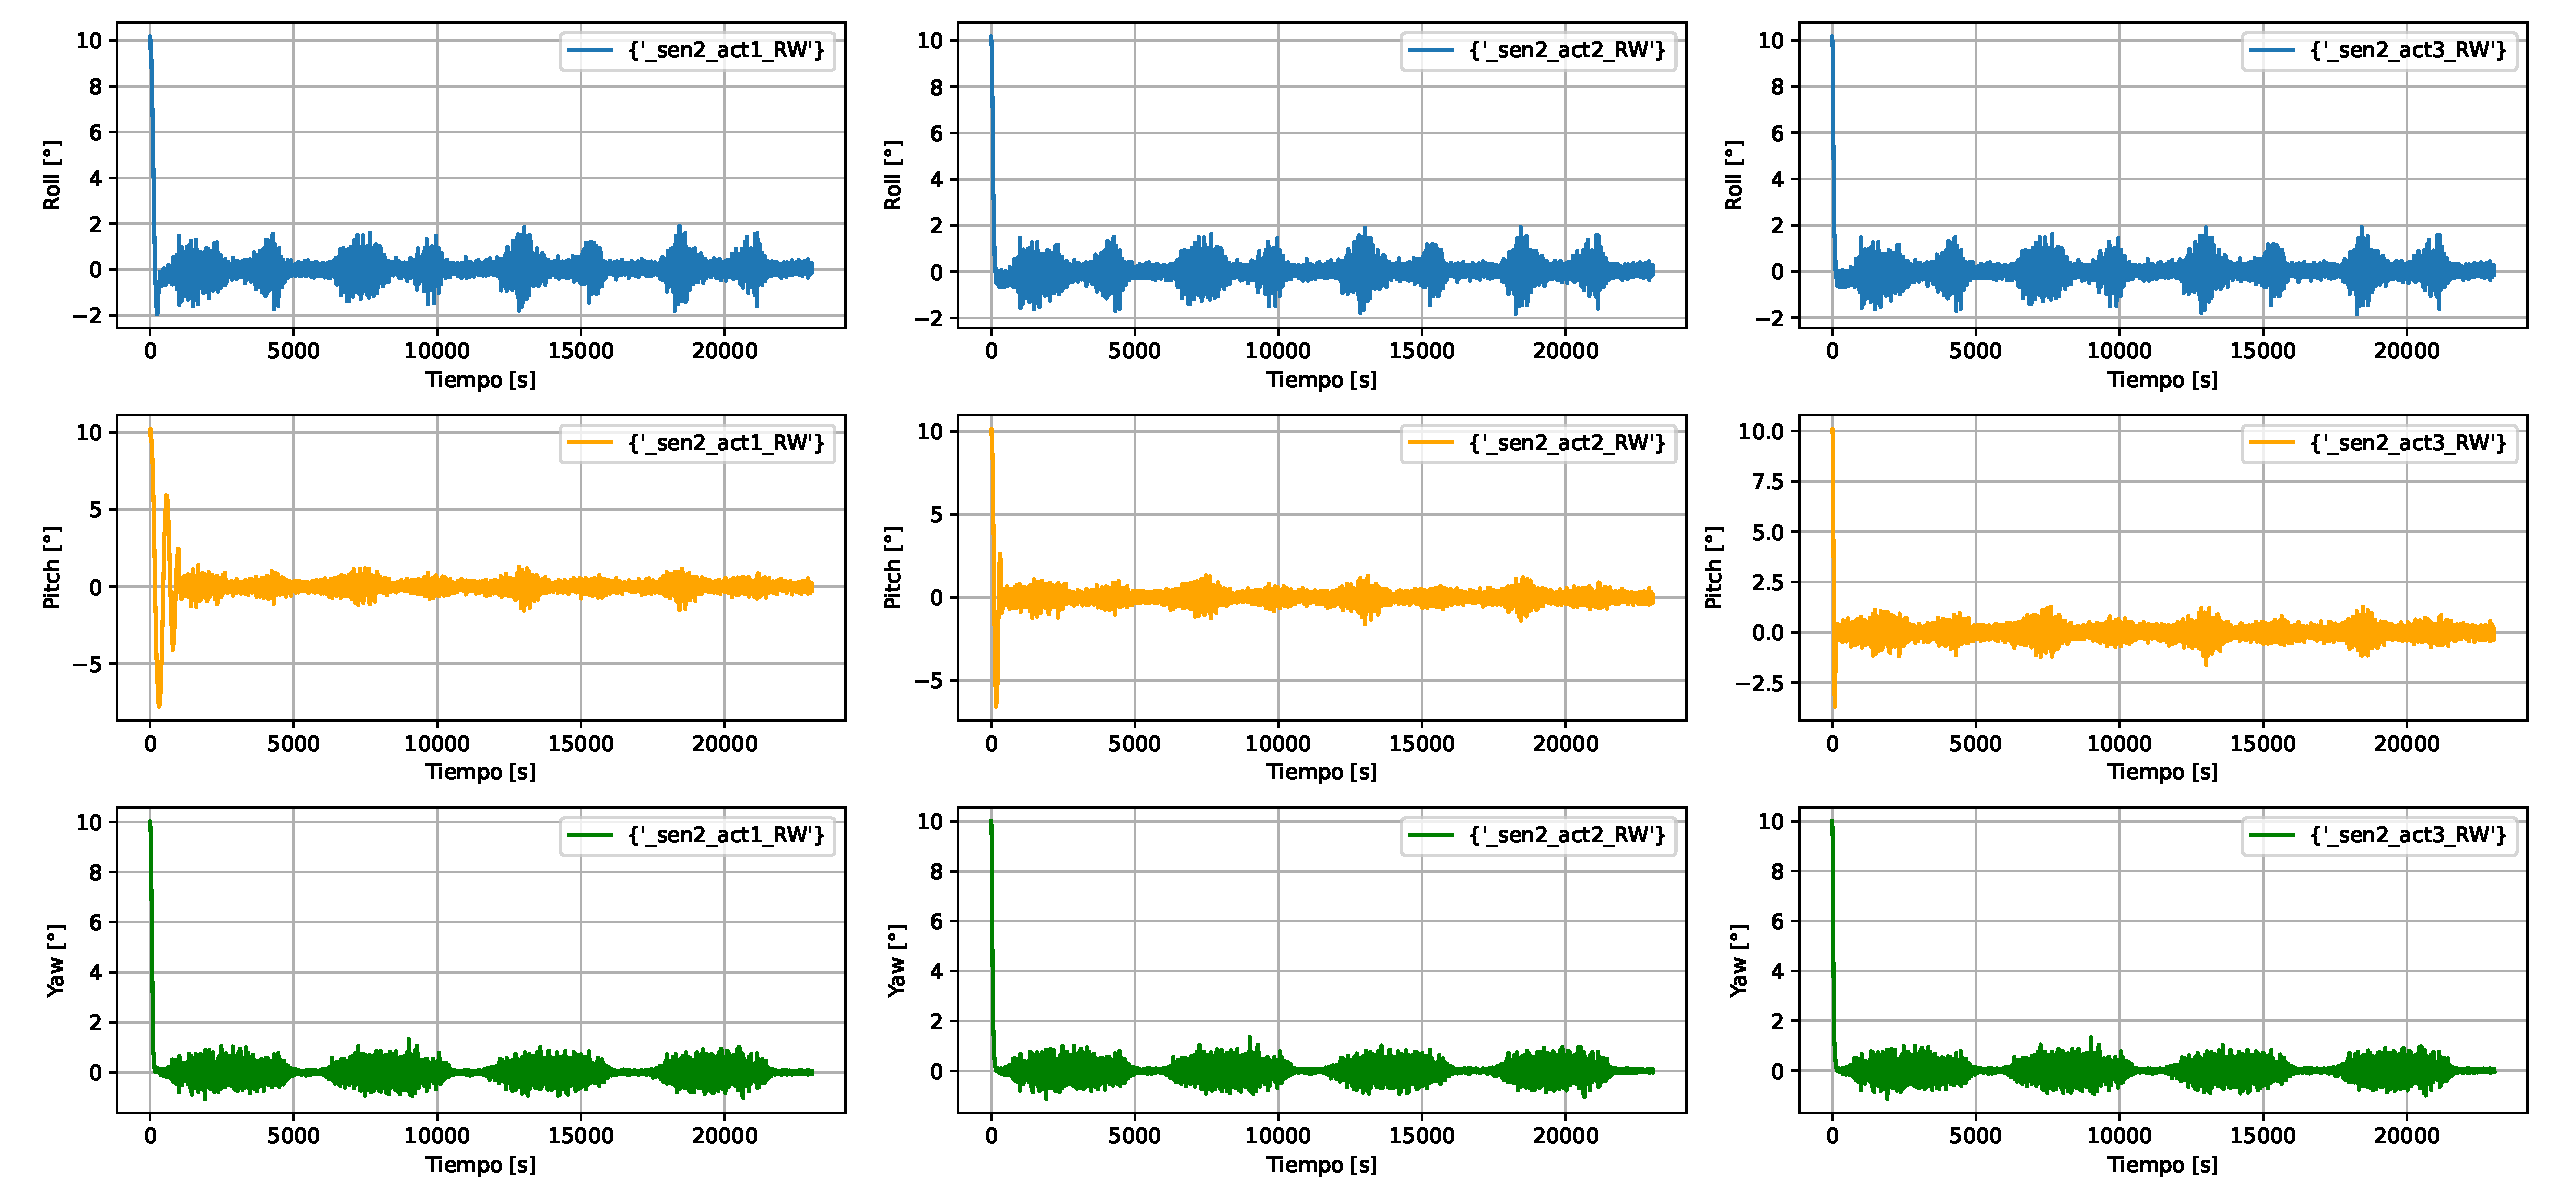
\includegraphics[width=0.97\textwidth]{RW_LQR_actuadores.pdf}
	\caption{Ángulos de Euler LVLH y body para niveles de rueda de reacción distintos con sensores nivel 2 (Elaboración propia).}
	\label{fig:RW_LQR_actuadores}
\end{figure}


\begin{table}[h!]
	\centering
	\caption{Rendimiento y costo para niveles de rueda de reacción con nivel 2 de sensor y LQR}
	\begin{tabular}{|c|c|c|c|c|c|}
		\hline
		\textbf{Nivel de}   & \textbf{Potencia} & \textbf{Masa [kg]} & \textbf{Accuracy [°]} & \textbf{Jitter} & \textbf{Agilidad [s]}  \\ 
		\textbf{sensor}  & \textbf{máxima [W]} & & & \textbf{[W/Hz]} &  \\
		\hline
		\textbf{Nivel 1}   & 6  & 0.75  & 1.18 & 0.36 & 628  \\
		&  &   &  &  &    \\
		\hline
		\textbf{Nivel 2}   & 9  & 0.95  & 0.93 & 0.16 & 228   \\
		& & & & &   \\
		\hline
		\textbf{Nivel 3}   & 10  & 3.2  & 0.95 & 0.15 & 63   \\
		& & & & &   \\
		\hline		
	\end{tabular}
	\label{tab:RW_LQR_actuadores}
\end{table}

\subsection{Resumen sobre rendimiento vs costo}